% WACV 2027 Applications Track draft, built from the official author kit.
\documentclass[10pt,twocolumn,letterpaper]{article}

\usepackage[review,applications]{wacv}
\usepackage{amsmath,amssymb,booktabs,multirow}
\usepackage{graphicx}
\usepackage{iftex}
\ifPDFTeX\else
  % Tectonic uses XeTeX locally; use the installed Times-compatible face.
  % Overleaf/pdfLaTeX continues to use the official WACV Times setup.
  \usepackage{fontspec}
  \setmainfont{Times New Roman}
\fi
\usepackage{microtype}
\usepackage{placeins}
\usepackage{xcolor}
\usepackage{enumitem}
\usepackage{mathtools}
\usepackage{pifont}
\usepackage{algorithm}
\usepackage{algpseudocode}
\usepackage{tikz}
\usetikzlibrary{arrows.meta,positioning,fit,calc,backgrounds}

% Result macros prevent unsupported claims from entering prose.
\newcommand{\tbd}[1]{\textit{[pending: #1]}}
\newcommand{\bestF}{\tbd{best cross-crop macro-F1}}
\newcommand{\deltaF}{\tbd{gain over uniform routing}}
\newcommand{\budgetSave}{\tbd{VLM-call reduction}}
\newcommand{\targetCoverage}{\tbd{coverage at target risk}}
\newcommand{\modelWinner}{\tbd{best compact model}}
\newcommand{\cmark}{\ding{51}}
\newcommand{\xmark}{\ding{55}}
\newcommand{\wacvtablefont}{\footnotesize}


\definecolor{wacvblue}{rgb}{0.21,0.49,0.74}
\usepackage[breaklinks,colorlinks,allcolors=wacvblue]{hyperref}

\def\wacvPaperID{2841}
\def\confName{WACV}
\def\confYear{2027}

\title{OrnaScout: Budget-Aware UAV Visual Evidence Selection for Reliable\\
Cross-Crop Nursery Monitoring with Compact Vision--Language Models}

\author{Anonymous WACV submission}

\begin{document}
\maketitle
\begin{abstract}
High-resolution UAV imagery offers a scalable basis for nursery inventory, but it is poorly matched to the fixed visual context of compact vision--language models (VLMs). A single 5K frame may contain hundreds of small plants; whole-image downsampling removes instance detail, whereas exhaustive overlapping tiles repeatedly process the same regions and make inference cost grow with image size. Transfer across ornamental crops is also difficult because canopy geometry, spacing, object scale, and background composition change substantially. We introduce \emph{OrnaScout}, a budget-aware framework that allocates a fixed visual-computation budget to cross-crop nursery monitoring. Splitting precedes tiling to prevent source leakage. A supervised detector provides local evidence; the Budgeted Evidence Selector combines score-based exploitation with controlled exploration to retain the same number of tiles for every VLM. A schema-constrained decoder produces auditable records, and a validation-fitted gate routes unsupported records to human review. We study 418 relabeled Azalea and Magnolia images containing 29,842 plant instances and 14,630 source-safe tiles. Azalea has a median of 97 plants per image versus 57 for Magnolia, and its median normalized box area is 44.1\% smaller. In a source-level validation audit at an eight-tile budget, count-ranked selection retained 45.5\% of annotated evidence, compared with 35.2\% for random selection. Exploit--explore routing retained 43.9\%, reduced overlap redundancy by 22.7\% relative to combined-score top-$K$, and increased hard-negative retention from 0.7\% to 6.7\%. These results expose a trade-off among foreground recall, spatial diversity, and negative evidence, establishing an equal-budget protocol for cross-crop VLM and selective-risk evaluation.
\end{abstract}

\section{Introduction}
Nursery scouting from unmanned aerial vehicles (UAVs) is a high-resolution, small-object problem. A single RGB frame may contain many repeated plants, uneven spacing, partial crowns, shadows, ground fabric, and row-edge truncation. Conventional detectors can localize and count annotated instances, but their output does not directly express scouting state, confidence, or the need for human review. General-purpose VLMs provide a richer interface, yet whole-image inference is poorly matched to 5K aerial imagery: downsampling erases small instances, exhaustive tiling is expensive, and free-form responses can remain syntactically valid while being visually unsupported. Prior edge-deployed UAV systems further motivate bounded inference when sensing and control must operate under finite onboard resources~\cite{kode2026drone}.

This work studies a narrower and falsifiable problem. Given a fixed budget of VLM calls per source image, can detector evidence identify informative regions, and can a validation-calibrated gate reduce unsupported compact-VLM decisions when the crop changes? The distinction matters. The detector supplies localized evidence; the VLM is responsible for a constrained semantic record; and the gate decides whether that record is reliable enough to use. None of these components is treated as an agronomic authority.

The evaluation uses two visually and geometrically different ornamental crops, Magnolia and Azalea. The relabeled corpus contains 297 Magnolia and 121 Azalea source images, with 15,644 and 14,198 usable boxes, respectively. Azalea has a higher median instance count (97 versus 57 plants per image) and a 44.1\% smaller median normalized box area. The crops also differ in greenness and spatial arrangement. We therefore treat crop identity as a domain shift rather than randomly mixing all tiles before splitting.

Our contributions are:
\begin{itemize}[leftmargin=*,nosep]
    \item a Budgeted Evidence Selector for high-resolution aerial imagery that combines detector confidence and clipped local count while preserving an explicit exploration fraction;
    \item a structured compact-VLM scouting task with hard-negative evaluation, repeated-generation consistency, and schema-level failure measurements;
    \item a validation-only selective gate evaluated through risk--coverage analysis rather than a single confidence threshold; and
    \item a source-safe cross-crop protocol with clustered confidence intervals, transfer matrices, edge-oriented latency and memory measurements, and equal-budget ablations.
\end{itemize}

The intended claim is algorithmic, not merely agricultural: localized evidence should be used to allocate scarce multimodal computation, and unsupported outputs should be reviewable rather than silently accepted.

\begin{figure*}[t]
    \centering
    \resizebox{\textwidth}{!}{\begin{tikzpicture}[
  font=\sffamily\scriptsize,
  box/.style={draw=black!68, rounded corners=1.2pt, align=center,
    minimum height=9mm, text width=22mm, inner sep=2.5pt},
  compact/.style={box, text width=19mm, minimum height=8mm, inner sep=2pt},
  data/.style={box, fill=blue!5},
  prep/.style={box, fill=cyan!7},
  evidence/.style={box, fill=green!7},
  select/.style={compact, fill=orange!10, draw=orange!72!black},
  vlm/.style={box, fill=violet!7, draw=violet!62!black},
  reliable/.style={box, fill=teal!8, draw=teal!65!black},
  outputbox/.style={compact, fill=gray!6},
  sample/.style={draw=black!70, line width=.45pt, inner sep=0pt, fill=white},
  stage/.style={draw=black!45, dashed, rounded corners=2pt,
    inner xsep=1.4mm, inner ysep=2.5mm},
  flow/.style={-{Latex[length=1.9mm,width=1.35mm]}, line width=.7pt, draw=black!78},
  train/.style={flow,dashed, draw=black!58},
  junction/.style={circle, fill=black!78, inner sep=0pt, minimum size=1.15mm}
]

% Row 1: real cross-crop inputs, source-safe preparation, and local evidence.
\node[sample] (magback) {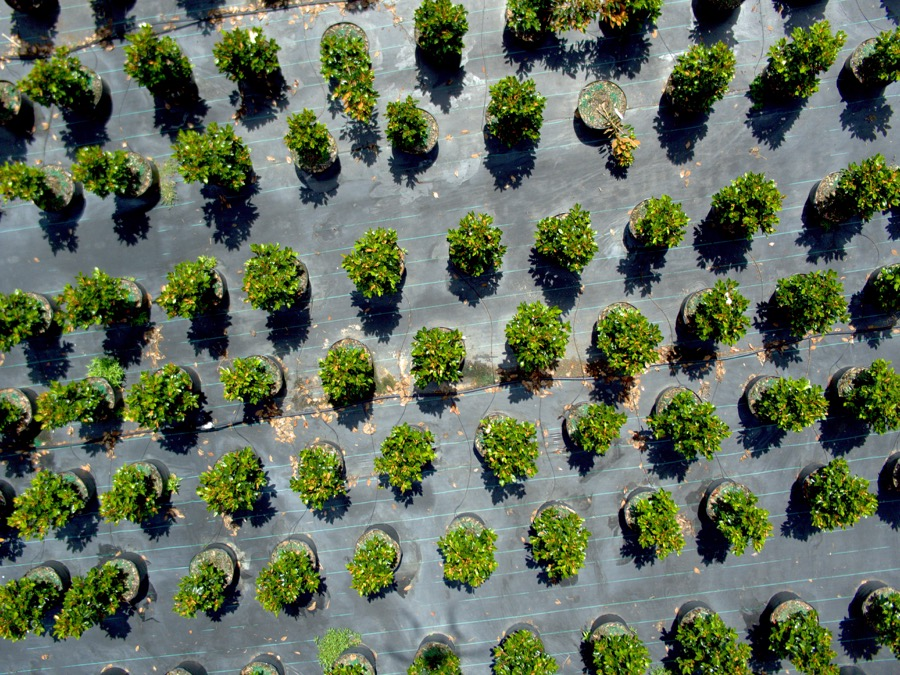
\includegraphics[width=20mm,height=15mm]{figures/input_examples/magnolia_03.jpg}};
\node[sample, xshift=-1.6mm, yshift=1.4mm] at (magback.center) (magmid)
  {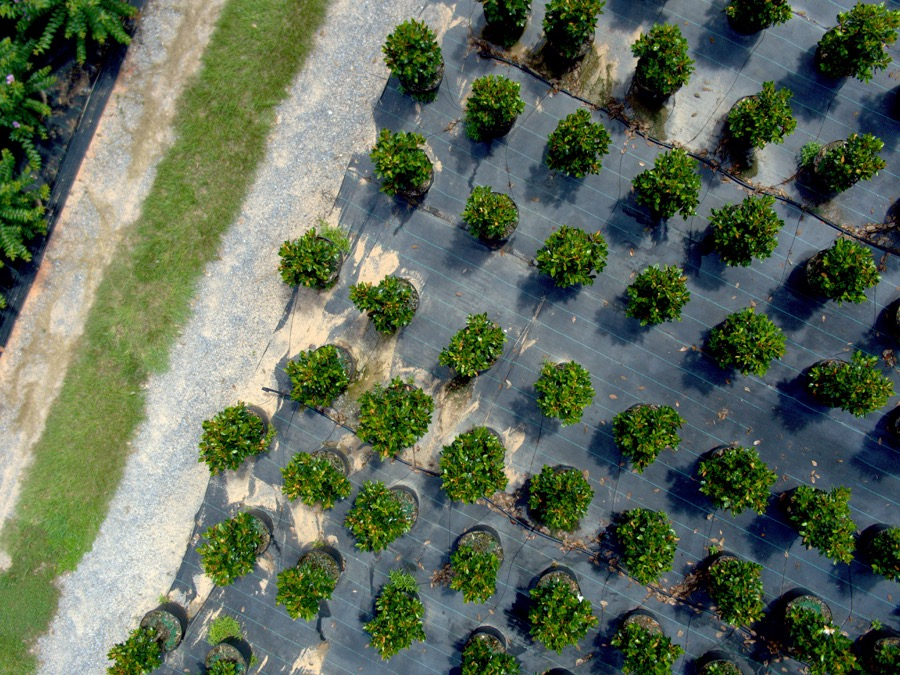
\includegraphics[width=20mm,height=15mm]{figures/input_examples/magnolia_02.jpg}};
\node[sample, xshift=-1.6mm, yshift=1.4mm] at (magmid.center) (mag)
  {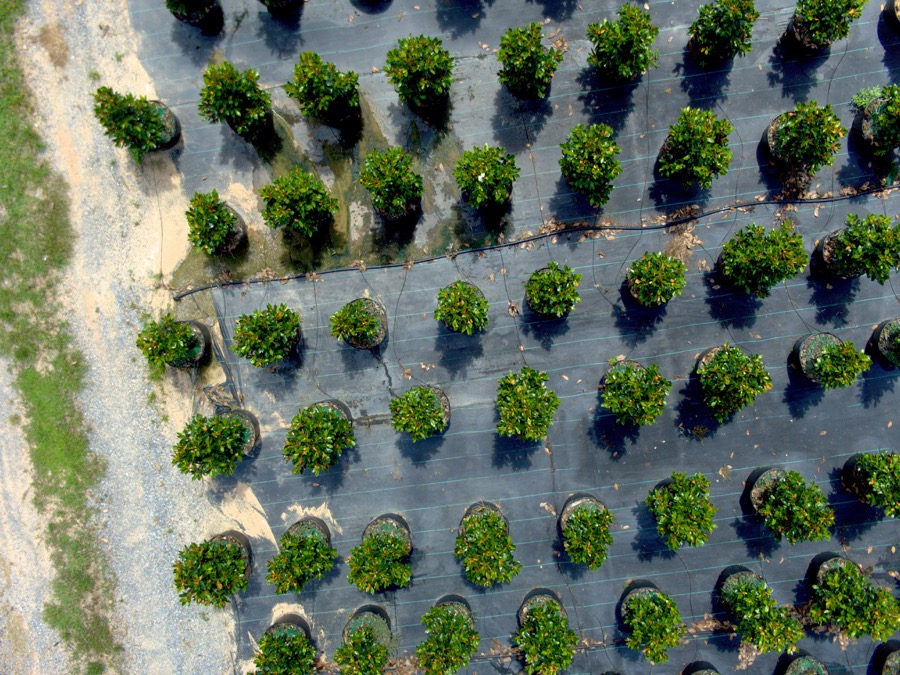
\includegraphics[width=20mm,height=15mm]{figures/input_examples/magnolia_01.jpg}};
\node[fit=(magback)(magmid)(mag), inner sep=.4mm] (magstack) {};
\node[font=\bfseries\scriptsize, above=.7mm of magstack] (maglabel) {Magnolia RGB};

\node[sample, below=8mm of magback] (azaback)
  {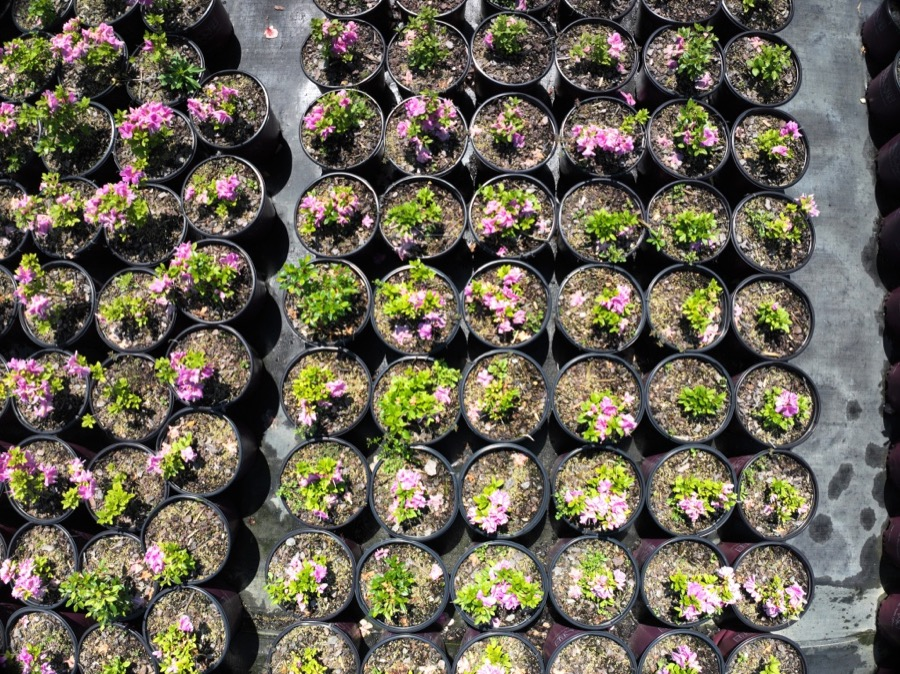
\includegraphics[width=20mm,height=15mm]{figures/input_examples/azalea_03.jpg}};
\node[sample, xshift=-1.6mm, yshift=1.4mm] at (azaback.center) (azamid)
  {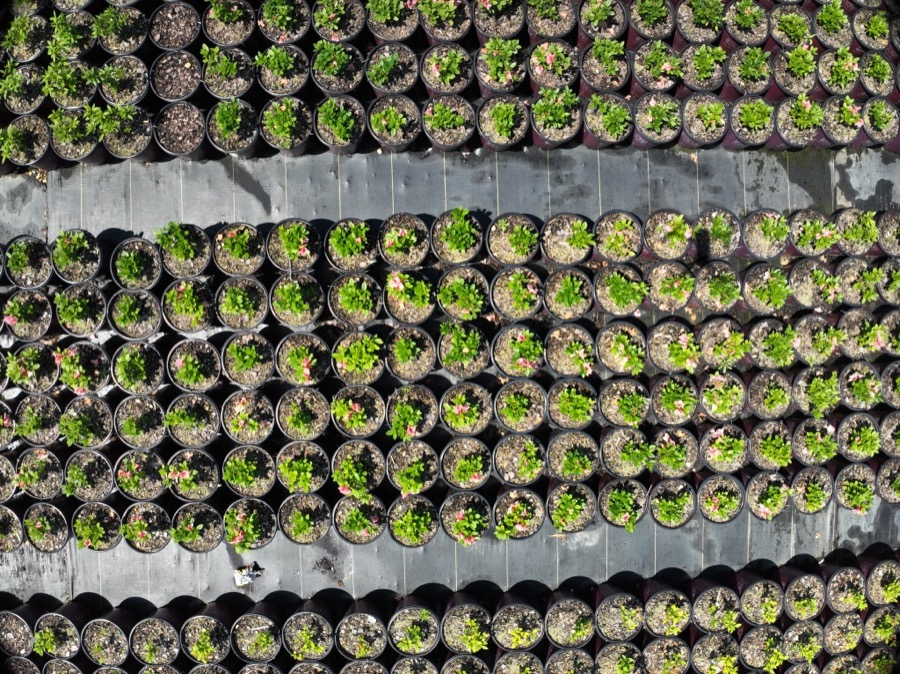
\includegraphics[width=20mm,height=15mm]{figures/input_examples/azalea_02.jpg}};
\node[sample, xshift=-1.6mm, yshift=1.4mm] at (azamid.center) (aza)
  {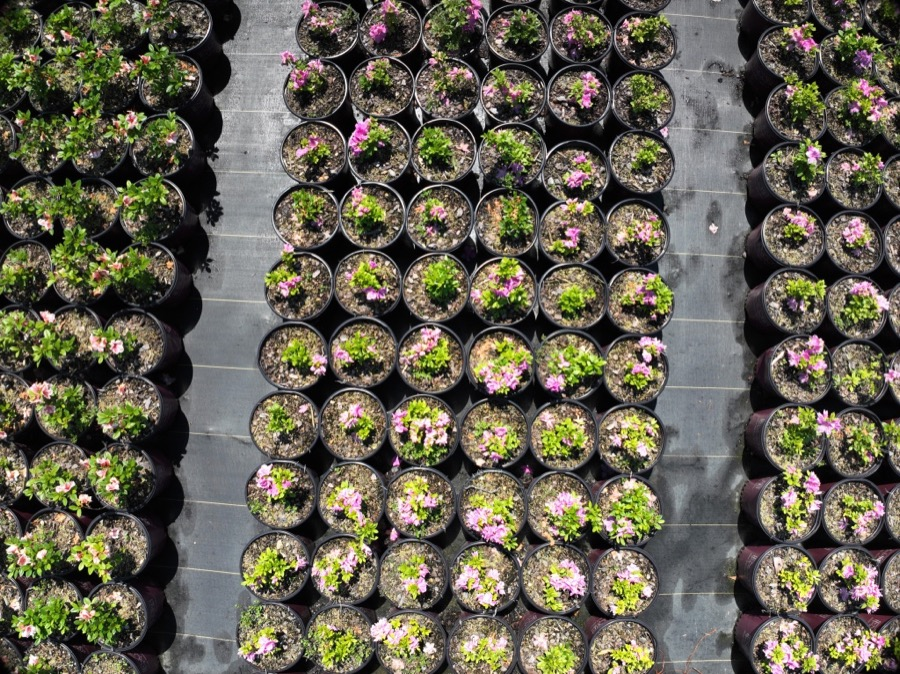
\includegraphics[width=20mm,height=15mm]{figures/input_examples/azalea_01.jpg}};
\node[fit=(azaback)(azamid)(aza), inner sep=.4mm] (azastack) {};
\node[font=\bfseries\scriptsize, above=.7mm of azastack] (azalabel) {Azalea RGB};

\node[prep, right=6mm of $(magstack.east)!0.5!(azastack.east)$] (split)
  {\textbf{Source split}\\train / val / test\\before tiling};
\node[prep, right=5mm of split] (tile)
  {\textbf{Overlapping tiles}\\$s\!\times\!s$, overlap $\alpha$};
\node[evidence, right=5mm of tile] (det)
  {\textbf{Detector evidence}\\confidence $c_t$\\count $n_t$};
\node[outputbox, right=5mm of det, fill=yellow!12, draw=orange!68!black] (labels)
  {\textbf{One-class boxes}\\training / scoring only};

% Row 2: selector, structured inference, and selective output.
\node[select, below=11mm of azastack] (rank)
  {\textbf{Evidence rank}\\$q_t=c_t+\bar n_t$};
\node[select, right=4mm of rank] (allocate)
  {\textbf{Allocate}\\top $K_x$ + explore $K_e$};
\node[select, right=4mm of allocate] (union)
  {\textbf{Budget union}\\$|\mathcal{S}_i|\leq K$};
\node[vlm, right=6mm of union] (adapter)
  {\textbf{VLM adapter}\\SmolVLM2 / Phi\\LLaVA};
\node[vlm, right=4mm of adapter] (schema)
  {\textbf{Schema decoder}\\fixed fields; no\\silent repair};
\node[reliable, right=5mm of schema] (signals)
  {\textbf{Reliability evidence}\\schema, repeats,\\detector agreement};
\node[reliable, right=4mm of signals] (gate)
  {\textbf{Failure-risk gate}\\validation-fitted\\threshold $\tau^*$};
\node[outputbox, right=4mm of gate, fill=green!8, draw=green!55!black] (accept)
  {\textbf{Accept}\\retain record};
\node[outputbox, below=3mm of accept, fill=orange!9, draw=orange!68!black] (review)
  {\textbf{Review}\\abstain / inspect};
\node[outputbox, below=5mm of gate, text width=22mm] (val)
  {\textbf{Validation outcomes}\\observed task failures};

% Boundary-to-boundary paths.
\draw[flow] (magstack.east) -- ++(1.4mm,0) |- ($(split.west)+(0,2mm)$);
\draw[flow] (azastack.east) -- ++(3.0mm,0) |- ($(split.west)+(0,-2mm)$);
\draw[flow] (split.east) -- (tile.west);
\draw[flow] (tile.east) -- (det.west);
\draw[train] (labels.west) -- (det.east);
\coordinate (selectorlane) at ($(rank.north)+(0,2.2mm)$);
\draw[flow] (det.south) |- (selectorlane) -- (rank.north);
\draw[flow] (rank.east) -- (allocate.west);
\draw[flow] (allocate.east) -- (union.west);
\draw[flow] (union.east) -- (adapter.west);
\draw[flow] (adapter.east) -- (schema.west);
\draw[flow] (schema.east) -- (signals.west);
\draw[flow] (signals.east) -- (gate.west);
\node[junction] (gatebranch) at ($(gate.east)+(2mm,0)$) {};
\draw[line width=.7pt, draw=black!78] (gate.east) -- (gatebranch);
\draw[flow] (gatebranch) -- (accept.west);
\draw[flow] (gatebranch) |- (review.west);
\draw[train] (val.north) -- node[right,font=\tiny]{fit on val only} (gate.south);

\begin{scope}[on background layer]
  \node[stage, fit=(maglabel)(magstack)(azalabel)(azastack)(split)(tile)] (stageA) {};
  \node[stage, fit=(det)(labels)] (stageB) {};
  \node[stage, fit=(rank)(allocate)(union), draw=orange!72!black] (stageC) {};
  \node[stage, fit=(adapter)(schema), draw=violet!55!black] (stageD) {};
  \node[stage, fit=(signals)(gate)(accept)(review)(val), draw=teal!55!black] (stageE) {};
\end{scope}

% Stage headings are independent of the dashed frames so text never touches a boundary.
\node[font=\bfseries\scriptsize, above=1.1mm of stageA.north]
  {A. Source-safe preparation};
\node[font=\bfseries\scriptsize, above=1.1mm of stageB.north]
  {B. Local evidence};
\node[font=\bfseries\scriptsize, text=orange!55!black, below=1.1mm of stageC.south]
  {C. Budgeted Evidence Selector};
\node[font=\bfseries\scriptsize, text=violet!40!black, below=1.1mm of stageD.south]
  {D. Structured VLM inference};
\node[font=\bfseries\scriptsize, text=teal!38!black, above=1.1mm of stageE.north]
  {E. Selective reliability};
\end{tikzpicture}
}
    \caption{\textbf{OrnaScout overview.} Source images are partitioned before tiling. Detector confidence and clipped local count rank candidate tiles; the proposed selector combines top-ranked exploitation with controlled exploration under a fixed budget $K$. A model adapter and fixed-schema decoder produce auditable task records. Reliability signals enter a failure-risk gate fitted only on validation outcomes; accepted records are retained and the remainder are referred for review. Solid arrows denote test-time computation and dashed arrows denote supervision or validation-only fitting.}
    \label{fig:architecture}
\end{figure*}

\section{Related Work}
\paragraph{Vision--language foundations and compact inference.}
Contrastive vision--language pretraining established transferable image--text representations~\cite{radford2021clip}; later systems introduced caption bootstrapping~\cite{li2022blip}, interleaved few-shot learning~\cite{alayrac2022flamingo}, frozen-backbone query transformers~\cite{li2023blip2}, and instruction tuning~\cite{dai2023instructblip,liu2023llava,liu2024llava15}. Compact deployments expose a different bottleneck: visual resolution and token count can dominate latency even when the language backbone is small. Phi-3.5-Vision and SmolVLM2 provide practical compact baselines~\cite{microsoft2024phi35vision,huggingface2025smolvlm2}, while FastVLM, NVILA, and learned token reduction study the accuracy--latency frontier more directly~\cite{vasu2025fastvlm,liu2025nvila,zhao2025token}. OrnaScout does not propose another VLM backbone; it allocates a fixed number of calls to spatial evidence and adds selective prediction around any compatible compact VLM.

\paragraph{VLM evaluation in specialized and aerial domains.}
AgEval demonstrated both the promise and class-dependent variability of general VLMs on plant-stress tasks~\cite{arshad2025ageval}. Aerial Mirage documented unsupported caption content in drone imagery~\cite{basak2025aerial}, and causal probing shows that scene context can trigger visual hallucinations~\cite{huang2025frisbee}. Active VLM selection~\cite{safaei2025activevlm} and human-centered benchmark design~\cite{jiang2025atbench} further motivate measuring uncertainty, task utility, and efficiency together. WACV efficiency studies caution that parameter count alone is not an adequate deployment metric~\cite{nauen2025transformer}. Our setting combines these concerns: high-resolution aerial evidence, structured output, explicit hard negatives, fixed compute, and crop-level transfer.

\paragraph{High-resolution detection and domain shift.}
UAV benchmarks such as UAVDT and VisDrone exposed the scale, density, and viewpoint difficulties of aerial detection~\cite{du2018uavdt,zhu2018visdrone}. Sparse high-resolution querying~\cite{yang2022querydet}, sliced inference~\cite{akyon2022sahi}, and spectral enhancement~\cite{sun2025set} reduce wasted computation or strengthen tiny-object features. Classical one-stage and set-prediction detectors remain useful evidence producers~\cite{redmon2016yolo,carion2020detr}. However, aerial deployment is sensitive to acquisition and scene shift. Frequency disentanglement improves generalized UAV detection~\cite{wang2023uav}; active learning reduces UAV annotation cost~\cite{yamani2024activeuav}; and recent benchmarks and algorithms study realistic remote-sensing or single-domain shifts~\cite{alemadi2025shift,danish2024dg,zhang2024csu}. Style-guided prompt learning likewise targets generalizable VLM features~\cite{talemi2025stylepro}. These methods motivate crop-disjoint transfer, but none evaluates a detector-routed compact VLM under a fixed per-image budget.

\paragraph{Generalization, calibration, and selective prediction.}
Domain-adversarial learning~\cite{ganin2016dann}, standardized domain-generalization evaluation~\cite{gulrajani2021domainbed}, and flat-minima selection~\cite{cha2021swad} all show that evaluation design is inseparable from generalization claims. Neural confidence is often miscalibrated~\cite{guo2017calibration}; selective classification therefore evaluates accuracy as coverage changes~\cite{geifman2017selective}, while SelectiveNet learns prediction and rejection jointly~\cite{geifman2019selectivenet}. Conformal risk control offers stronger guarantees under appropriate assumptions~\cite{angelopoulos2024crc}, and uncertainty evaluation must distinguish ranking quality from raw confidence~\cite{ding2020uncertainty}. Our gate is deliberately described as empirical validation calibration: it does not claim distribution-free coverage after crop shift.

\paragraph{Agricultural context.}
UAV sensing and deep learning are established tools in precision agriculture~\cite{zhang2012uav,osco2021precision}. WeedsGalore illustrates both the value and annotation cost of dense UAV crop imagery~\cite{celikkan2025weedsgalore}. Recent ornamental studies have examined annotation-free counting under color and domain variation~\cite{manjunatha2026beyondgreen}, while temporal UAV cotton analysis has explored hybrid feature selection for condition discrimination~\cite{manjunatha2026agriqfs}. AgroGPT shows how agricultural supervision can specialize multimodal models~\cite{awais2025agrogpt}. Separately, UAV rose-bloom analysis demonstrates the practical value of tiling and localized language summaries for nursery imagery~\cite{sundaravadivel2026rosai}. The present work instead makes cross-crop transfer, compute allocation, and abstention the primary computer-vision problem. It neither constructs an agricultural foundation model nor treats language generation as an unverified terminal report.

\section{Method}
\subsection{Problem setup and scientific scope}
Let a source UAV image be $I_i$ with crop domain $d_i\in\{\mathrm{Magnolia},\mathrm{Azalea}\}$ and one-class instance boxes $\mathcal{B}_i$. These boxes supervise detector training and define evaluation targets; they are not exposed to the VLM during validation or testing. A tiling operator $\mathcal{T}_{s,\alpha}$ produces candidate tiles of side length $s$ and overlap $\alpha$. Source images are assigned to train, validation, or test partitions before tiling, so correlated tiles cannot cross partitions.

For each source image, the system may submit at most $K$ tiles to a VLM. Its output is a fixed-schema scouting record containing plant presence, count bin, density, coverage, visible evidence, priority, confidence, and a review flag. The problem is selective task prediction under two constraints: a visual-computation budget and a crop-domain shift. It is not unrestricted caption generation and does not infer disease or management labels absent from the annotations.

\subsection{Local detector evidence}
A lightweight detector trained on source-safe training tiles returns detections $\mathcal{D}_t$ for tile $t$. We retain the number of predictions $n_t=|\mathcal{D}_t|$ and their mean confidence $c_t$. The implemented ranking score is
\begin{equation}
q_t=c_t+\frac{\min(n_t,n_{\max})}{n_{\max}},\qquad n_{\max}=20.
\label{eq:evidence}
\end{equation}
The confidence term favors visually supported tiles; clipping prevents unusually dense regions from dominating the rank solely through count. The deliberately small evidence model makes the routing decision inspectable and permits confidence-only and count-only ablations.

Following the use of hard examples to suppress persistent detector errors \cite{shrivastava2016ohem}, we additionally evaluate one training-only hard-negative mining round. Detector responses from training images are matched against the training annotations, and unmatched regions containing no labeled plant are incorporated as empty-label negatives during retraining. This refinement changes the detector evidence supplied to the selector, but it introduces no additional component into the test-time OrnaScout architecture.

\subsection{Budgeted Evidence Selector}
For candidate set $\mathcal{T}_i$, the selector allocates $K_e=\operatorname{round}(\rho K)$ exploration slots and $K_x=K-K_e$ exploitation slots. Exploitation retains the $K_x$ largest values of Eq.~\eqref{eq:evidence}; exploration samples without replacement from the remaining tiles using a fixed seed:
\begin{align}
\mathcal{X}_i &= \operatorname{TopK}_{K_x}(\mathcal{T}_i;q), \\
\mathcal{E}_i &\sim \operatorname{Sample}_{K_e}(\mathcal{T}_i\setminus\mathcal{X}_i), \\
\mathcal{S}_i &= \mathcal{X}_i\cup\mathcal{E}_i,\qquad |\mathcal{S}_i|\le K.
\label{eq:router}
\end{align}
The exploration branch limits dependence on detector calibration and retains a chance of observing low-ranked but informative regions. Random, spatially uniform, and pure top-$K$ policies use the same $K$; consequently, differences measure evidence allocation rather than additional VLM input.

\subsection{Source-level evidence audit}
We evaluate routing before asking whether a VLM answers correctly. This separation is useful because a selector can fail by withholding relevant visual evidence even when the downstream model is capable. Let $b_j\in\mathcal{B}_i$ be an original source-image box and $v(b_j,t)\in[0,1]$ the fraction of its area visible in tile $t$. At visibility threshold $\eta=.5$, evidence recall is
\begin{equation}
R_{\mathrm{evid}}(i)=\frac{1}{|\mathcal{B}_i|}
\sum_{b_j\in\mathcal{B}_i}\mathbb{1}\!\left[
\max_{t\in\mathcal{S}_i}v(b_j,t)\ge\eta\right].
\label{eq:evidence-recall}
\end{equation}
Boxes are counted once in source coordinates, avoiding duplicate credit from overlapping tiles. We also measure spatial coverage
\begin{equation}
C_{\mathrm{sp}}(i)=
\frac{\left|\bigcup_{t\in\mathcal{S}_i}\Omega_t\right|}{|\Omega_i|},
\label{eq:spatial-coverage}
\end{equation}
and overlap redundancy
\begin{equation}
D_{\mathrm{red}}(i)=
\frac{\sum_{t\in\mathcal{S}_i}|\Omega_t|}
{\left|\bigcup_{t\in\mathcal{S}_i}\Omega_t\right|}-1.
\label{eq:redundancy}
\end{equation}
Boundary truncation is the fraction of covered instances whose maximum visible fraction lies in $[\eta,.98)$. Hard-negative recall records the proportion of available empty tiles retained by the selector. A ground-truth oracle and a shuffled-score selector are diagnostic controls only: neither is a deployable method.

\begin{algorithm}[t]
\caption{Budgeted routing and selective VLM inference}
\label{alg:ornascout}
\begin{algorithmic}[1]
\Require Image $I_i$; detector $f_D$; VLM $f_V$; budget $K$; exploration $\rho$; gate $h_{\tau^*}$
\Ensure Accepted records $\mathcal{A}_i$; review set $\mathcal{R}_i$
\State $\mathcal{T}_i\gets\mathcal{T}_{s,\alpha}(I_i)$
\ForAll{$t\in\mathcal{T}_i$}
  \State $(c_t,n_t)\gets f_D(t)$; compute $q_t$ using Eq.~\eqref{eq:evidence}
\EndFor
\State $K_e\gets\operatorname{round}(\rho K)$; $K_x\gets K-K_e$
\State $\mathcal{X}_i\gets\operatorname{TopK}_{K_x}(\mathcal{T}_i;q)$
\State $\mathcal{E}_i\gets\operatorname{Sample}_{K_e}(\mathcal{T}_i\setminus\mathcal{X}_i)$
\ForAll{$t\in\mathcal{X}_i\cup\mathcal{E}_i$}
  \State $z_t\gets\operatorname{DecodeSchema}(f_V(t,p))$
  \State $u_t\gets[s_{\mathrm{sch}},s_{\mathrm{con}},s_{\mathrm{det}},c_t^{\mathrm{vlm}}]$
  \If{$h_{\tau^*}(u_t)=\mathrm{accept}$}
    \State $\mathcal{A}_i\gets\mathcal{A}_i\cup\{z_t\}$
  \Else
    \State $\mathcal{R}_i\gets\mathcal{R}_i\cup\{(t,z_t)\}$
  \EndIf
\EndFor
\State \Return $\mathcal{A}_i,\mathcal{R}_i$
\end{algorithmic}
\end{algorithm}

\subsection{Model-agnostic structured inference}
Each $t\in\mathcal{S}_i$ and a frozen instruction $p$ are passed through one VLM adapter. The same image evidence, prompt, decoding budget, and schema are used for SmolVLM2, Phi-3.5-Vision, and LLaVA. The parser does not silently repair malformed responses. For a generation $z$, exact schema validity is
\begin{equation}
s_{\mathrm{sch}}(z)=\frac{1}{J}\sum_{j=1}^{J}\mathbb{1}\{g_j(z)=1\},\qquad J=9,
\label{eq:schema}
\end{equation}
where $g_j$ checks one required field or constraint. With $R>1$ generations, repeat consistency averages modal agreement over the five categorical task fields $\mathcal{F}$:
\begin{equation}
s_{\mathrm{con}}(t)=\frac{1}{|\mathcal{F}|}\sum_{k\in\mathcal{F}}
\frac{\max_v\sum_{r=1}^{R}\mathbb{1}[z_{t,r,k}=v]}{R}.
\label{eq:consistency}
\end{equation}
Detector agreement $s_{\mathrm{det}}$ measures agreement on presence and count bin when detector evidence is available.

\subsection{Evidence-calibrated selective decision}
An interpretable fixed baseline combines available evidence as
\begin{equation}
g_t=.35s_{\mathrm{sch}}+.25s_{\mathrm{con}}+.20c_t^{\mathrm{vlm}}+.20s_{\mathrm{det}},
\label{eq:fixedgate}
\end{equation}
with weights renormalized when a component is unavailable. The proposed gate fits a class-balanced logistic failure model on validation records only, using $[s_{\mathrm{sch}},s_{\mathrm{con}},s_{\mathrm{det}},g_t]$. If $\hat r_t$ is predicted error probability, the threshold is chosen before test evaluation:
\begin{equation}
\tau^*=\max_{\tau}\left\{\tau:
\frac{\sum_t\mathbb{1}[\hat r_t\le\tau]e_t}
{\max(1,\sum_t\mathbb{1}[\hat r_t\le\tau])}\le\epsilon\right\}.
\label{eq:threshold}
\end{equation}
Records with $\hat r_t>\tau^*$ are referred for review. This is empirical validation control, not a distribution-free guarantee under crop shift.

\subsection{Source-level reduction}
Tile records are grouped by source image for clustered uncertainty estimates. A deployable source record additionally requires a frozen overlap-aware reducer. Our planned reducer uses confidence-weighted voting over accepted records and coordinate-aware fusion of detector counts; a source with no accepted record is referred for review. Until that reducer is implemented and evaluated, we report tile-task results and source-clustered intervals, but no unsupported source-level accuracy.

\section{Experimental Design}
\subsection{Dataset construction and audit}
The relabeled snapshot contains 418 source images: 297 Magnolia and 121 Azalea. After rejecting five zero-width rows, 29,842 usable one-class annotations remain (15,644 Magnolia; 14,198 Azalea). Three reviewed Azalea images contain no instances and are retained as source-level negatives; one unlabeled Azalea RGB frame is excluded. Magnolia images are $5184\!\times\!3888$ and Azalea images are $5280\!\times\!3956$. With $s=1024$, $\alpha=.25$, and a minimum retained-box visibility of $.5$, preprocessing yields 14,630 tiles and 1,328 boundary-aware hard negatives.

\begin{table}[t]
\centering
\wacvtablefont
\caption{Relabeled corpus and source-safe tiling snapshot. Box statistics precede tiling.}
\label{tab:data}
\setlength{\tabcolsep}{5pt}
\begin{tabular}{lrrr}
\toprule
Crop & Sources & Boxes & Tiles \\
\midrule
Magnolia & 297 & 15,644 & 10,395 \\
Azalea & 121 & 14,198 & 4,235 \\
\midrule
Total & 418 & 29,842 & 14,630 \\
\bottomrule
\end{tabular}
\end{table}

A balanced human audit samples crop, source, box-size stratum, image boundary, and annotation-density stratum. Final detector and VLM results are released only after the audit size, agreement, and exclusion rules are frozen.

\subsection{Observed cross-crop shift}
Figure~\ref{fig:domainshift} describes the transfer setting before model fitting. Azalea contains a median of 97 boxes per image versus 57 for Magnolia, while its median normalized box area is $44.1\%$ smaller. Appearance and green-fraction marginals also differ. These statistics motivate crop-disjoint evaluation; they are not presented as a causal explanation of transfer error.

\begin{figure*}[t]
    \centering
    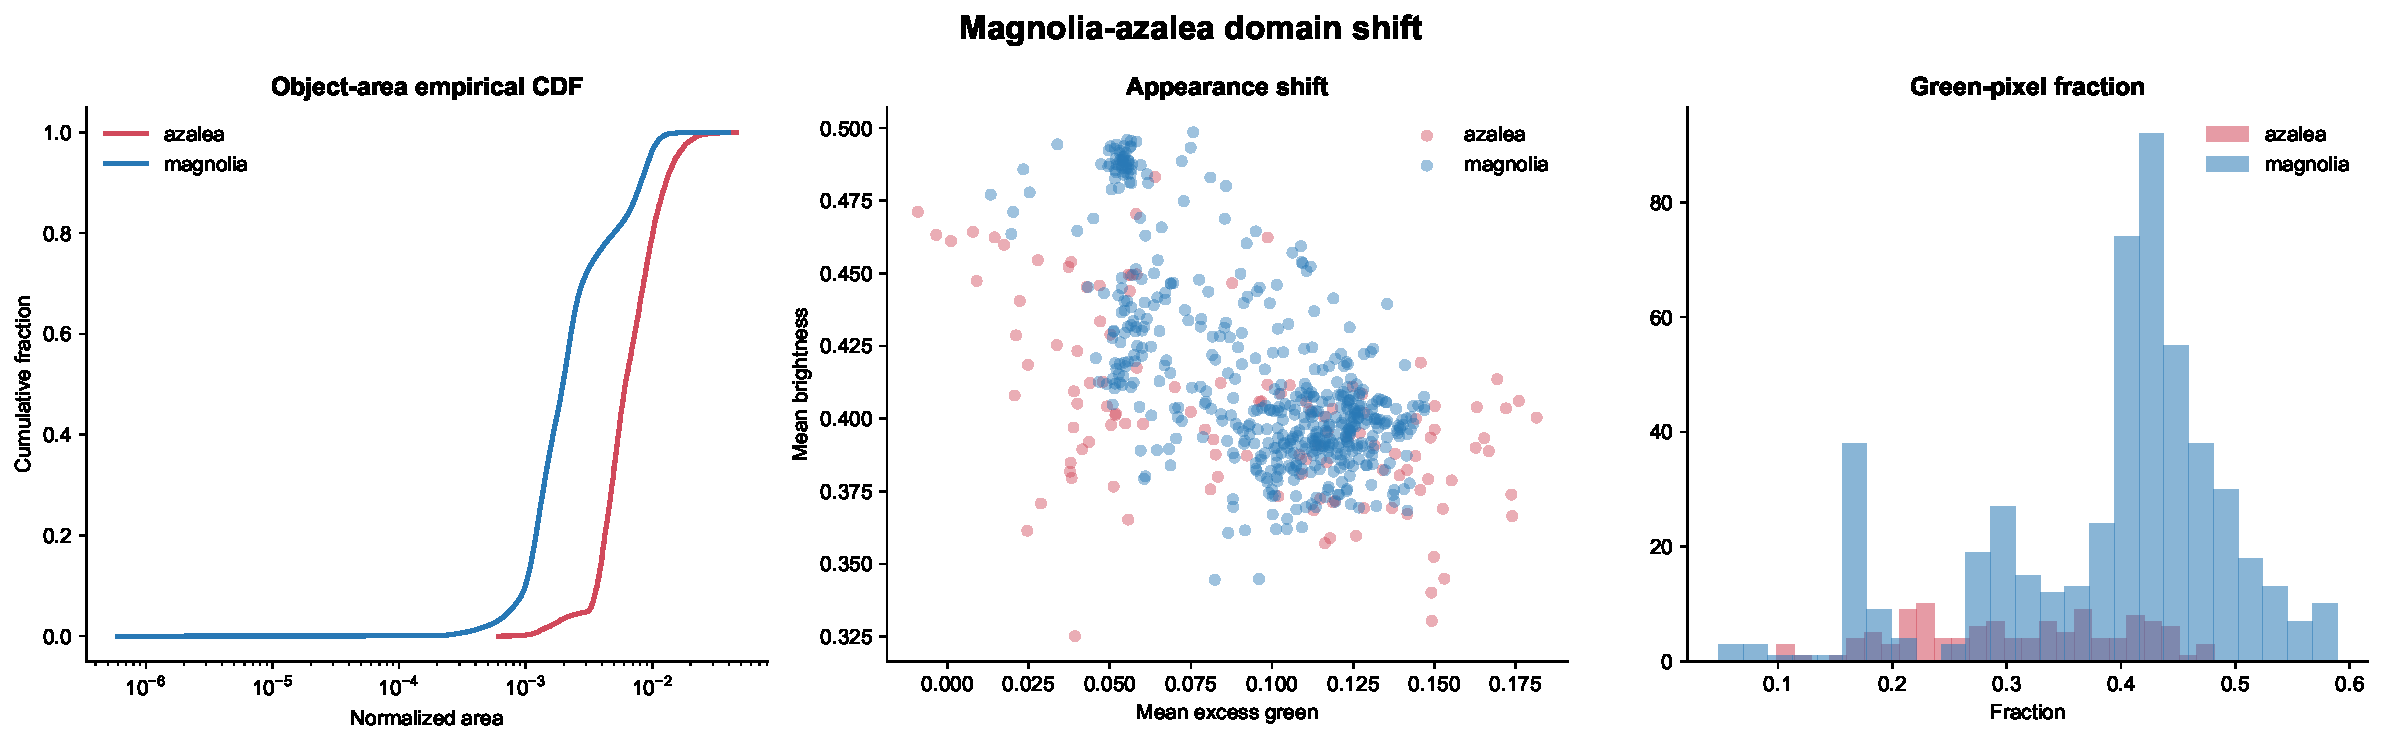
\includegraphics[width=\textwidth]{figures/cross_crop_shift.pdf}
    \caption{\textbf{Measured Magnolia--Azalea domain shift.} The object-area CDF uses valid ground-truth boxes; appearance statistics are computed once per source image. The differences in scale, density, and RGB appearance motivate directed cross-crop evaluation. No prediction is used in this figure.}
    \label{fig:domainshift}
\end{figure*}

\subsection{Source-safe evaluation protocols}
The fixed source split contains 302 training, 58 validation, and 58 test images, yielding 10,570, 2,030, and 2,030 tiles. We report five protocols: Magnolia$\rightarrow$Magnolia (M$\rightarrow$M), Azalea$\rightarrow$Azalea (A$\rightarrow$A), M$\rightarrow$A, A$\rightarrow$M, and crop-stratified pooled training. Target-crop test labels are used only for final scoring. Prompts, count bins, selector parameters, gate fitting, and checkpoint choice are frozen without test feedback.

\subsection{Models, task, and controlled baselines}
The model ladder comprises SmolVLM2-500M, SmolVLM2-2.2B, Phi-3.5-Vision, and LLaVA-1.5-7B. All models receive identical selected tiles, task schema, maximum generation length, and decoding settings. This is a model-generality study, not a claim that all four models have equal deployment cost.

Selector baselines are evaluated at the same $K$: random sampling, spatially uniform sampling, confidence-only top-$K$, count-only top-$K$, combined-score top-$K$ ($\rho=0$), and the full exploit--explore selector. Shuffled detector scores provide a negative control, while ground-truth-oracle routing is shown only as a diagnostic upper bound. Gate baselines are raw VLM confidence, schema-only rejection, the fixed weighted score in Eq.~\eqref{eq:fixedgate}, and the validation-fitted gate.

\paragraph{Detector training.}
The baseline and mined-negative variants use the same detector architecture, source split, image size, optimization schedule, augmentation policy, and validation protocol. Mining is confined to the training partition: predictions generated at confidence $.30$ are treated as unmatched when their maximum intersection over union with a training annotation is below $.30$. Candidate $1024\!\times\!1024$ crops containing any labeled plant are discarded, leaving 70 empty-label negatives for one retraining round. Checkpoint and threshold choices use validation data only, and the held-out test partition remains untouched. The separate held-out count output is not reported in this ablation because a matched baseline count run under the same post-processing configuration is unavailable.

\subsection{Metrics and statistical protocol}
Task performance is macro-F1 for presence, count bin, density, and coverage. Reliability is measured by exact schema-valid rate, hard-negative hallucination rate, false-accept rate, accepted risk at fixed coverage, coverage at a predeclared risk target, and area under the risk--coverage curve (AURC). For $N$ test records sorted by increasing predicted risk, $e_{(j)}\in\{0,1\}$ denotes whether the complete four-field task record is incorrect. We compute
\begin{equation}
R_m=\frac{1}{m}\sum_{j=1}^{m}e_{(j)},\qquad
\mathrm{AURC}=\frac{1}{N}\sum_{m=1}^{N}R_m.
\label{eq:aurc}
\end{equation}
Efficiency includes mean and p95 latency, peak resident memory, throughput, and VLM calls per source image. One unmeasured warm-up generation is performed before timing; the generation seed is deterministically derived from the frozen study seed, tile identifier, and repeat index.

All confidence intervals use 1,000 source-image cluster-bootstrap resamples. Tiles from a source image are resampled together. Model comparisons use paired bootstrap differences when the test sources coincide. Latency and memory are measured with the same hardware, software revision, precision, image resolution, warm-up, and generation length; model-loading memory is reported separately from incremental inference memory.

\subsection{Causal ablation plan}
The ablations mirror the method decomposition rather than varying unrelated settings:
\begin{enumerate}[leftmargin=*,nosep]
    \item \textbf{Ranking evidence:} confidence only, clipped count only, and their combination.
    \item \textbf{Allocation policy:} random, spatially uniform, pure top-$K$, and exploit--explore at fixed $K$.
    \item \textbf{Budget sensitivity:} $K\in\{1,2,4,8,16\}$ and $\rho\in\{0,.125,.25,.50,.75,1\}$.
    \item \textbf{Reliability evidence:} add schema validity, repeat consistency, detector agreement, and the validation-fitted gate sequentially.
    \item \textbf{Model generality:} repeat the frozen selector and gate protocol across all four VLMs.
\end{enumerate}
Tile size $s\in\{512,768,1024,1536\}$, overlap $\alpha\in\{0,.125,.25,.50\}$, prompt sensitivity, and one-versus-three-generation studies are reported in the supplement. Selector diagnostics use Eqs.~\eqref{eq:evidence-recall}--\eqref{eq:redundancy} at source-image level. Stochastic policies are repeated ten times and then averaged per source; 95\% intervals use 1,000 source-cluster bootstrap resamples.

\section{Results}
\paragraph{Reporting rule.}
Every value is imported from a versioned CSV artifact. Smoke tests establish compatibility only. The source-level selector audit below is a validation diagnostic used to freeze the routing protocol; VLM task, transfer, and selective-risk tables remain incomplete until the corresponding frozen runs finish.

\subsection{Dataset construction and shift}
Table~\ref{tab:data} records the audited data snapshot. Azalea is not a smaller copy of the Magnolia domain: it contains more labeled instances per source image but smaller normalized objects and a lower median green-pixel fraction (.312 versus .429). This measured shift defines the directed transfer experiment but does not itself establish robustness.

\paragraph{Effect of detector hard-negative mining.}
Table~\ref{tab:hnm} reports the matched validation comparison used to assess the detector refinement. One hard-negative mining round removed 101 false positives, an $11.6\%$ relative reduction, while AP$_{50{:}95}$ increased by $.011$. Precision and recall each increased by approximately $.006$. These changes indicate cleaner evidence entering OrnaScout; they are not attributed to the Budgeted Evidence Selector.

\begin{table}[t]
\centering
\wacvtablefont
\caption{Effect of one training-only hard-negative mining round on detector validation performance. Architecture, source split, optimization, augmentation, and evaluation settings are held fixed. False positives are measured by matching detections to validation annotations.}
\label{tab:hnm}
\setlength{\tabcolsep}{4.2pt}
\begin{tabular}{lrrrr}
\toprule
Detector training & AP$_{50{:}95}\uparrow$ & Prec.$\uparrow$ & Rec.$\uparrow$ & FP$\downarrow$ \\
\midrule
Baseline & .756 & .938 & .941 & 873 \\
+ one HNM round & \textbf{.767} & \textbf{.943} & \textbf{.947} & \textbf{772} \\
\bottomrule
\end{tabular}
\end{table}

\subsection{Selector ablation at equal budget}
Table~\ref{tab:selector} isolates the proposed selector using one primary VLM, fixed $K$, and identical decoding. The critical comparison is full exploit--explore routing against combined-score top-$K$: it tests whether reserved exploration contributes beyond detector ranking.
To isolate evidence allocation from gate fitting, AURC orders records with the fixed evidence score in Eq.~\eqref{eq:fixedgate}; no selector-specific threshold is fitted on the test set.

Before VLM inference, Table~\ref{tab:evidence-audit} tests whether each selector retains the annotated evidence at $B=8$. Count top-$K$ gives the highest evidence recall among deployable policies on validation ($.455$), narrowly ahead of combined top-$K$ ($.451$). Exploit--explore does not improve recall ($.439$), but reduces overlap redundancy and retains more hard-negative tiles than the detector-ranked policies. Spatially uniform selection attains similar recall with the broadest coverage and no tile overlap. These results prevent us from treating the proposed policy as uniformly superior; its value must be established by the downstream task and selective-risk experiments.

\begin{table}[t]
\centering
\wacvtablefont
\caption{Source-level validation audit at $B=8$. Evidence recall includes source-clustered 95\% CIs. GT oracle is diagnostic only.}
\label{tab:evidence-audit}
\setlength{\tabcolsep}{3.3pt}
\resizebox{\columnwidth}{!}{%
\begin{tabular}{lcccc}
\toprule
Selector & Evid. recall & Spatial cov. & Redund.$\downarrow$ & Hard-neg. rec. \\
\midrule
Random & $.352\;[.335,.382]$ & $.361$ & $.141$ & $.231$ \\
Spatial uniform & $.438\;[.415,.464]$ & $.411$ & $\mathbf{.000}$ & $.196$ \\
Confidence top-$K$ & $.384\;[.350,.425]$ & $.340$ & $.214$ & $.024$ \\
Count top-$K$ & $\mathbf{.455}\;[.420,.496]$ & $.330$ & $.252$ & $.015$ \\
Combined top-$K$ & $.451\;[.416,.494]$ & $.330$ & $.254$ & $.007$ \\
Exploit--explore & $.439\;[.410,.474]$ & $.345$ & $.196$ & $.067$ \\
Shuffled score & $.353\;[.336,.382]$ & $.361$ & $.142$ & $.236$ \\
GT oracle & $.506\;[.471,.544]$ & $.335$ & $.233$ & $.002$ \\
\bottomrule
\end{tabular}}
\end{table}

Figure~\ref{fig:selector-budget} reports the full budget sweep. Increasing $B$ predictably raises evidence recall and spatial coverage, but also increases redundant overlap. The curves are routing diagnostics, not VLM accuracy curves.

\begin{figure*}[t]
    \centering
    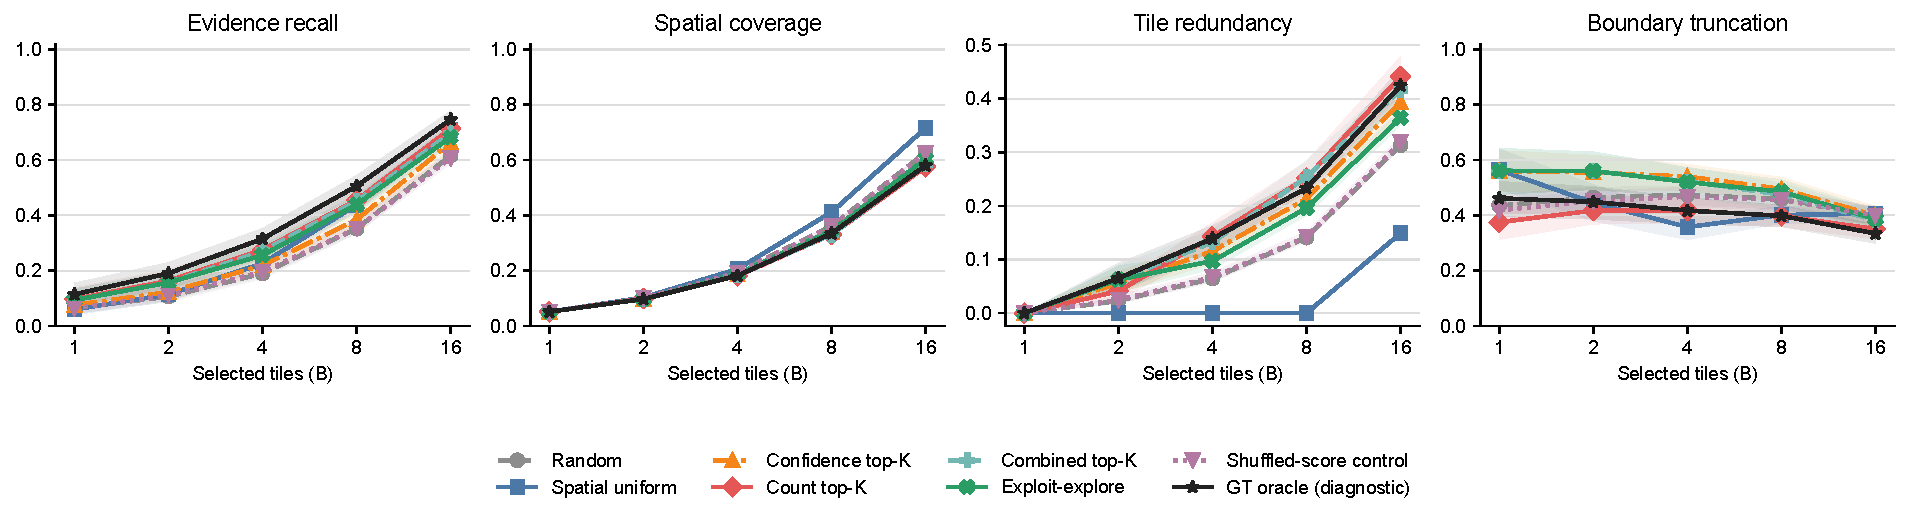
\includegraphics[width=\textwidth]{figures/selector_budget_audit_main.pdf}
    \caption{\textbf{Validation-only evidence audit across visual budgets.} Means and source-clustered 95\% bootstrap intervals are computed over 58 validation images. Random, exploit--explore, and shuffled-score policies are averaged over ten deterministic repetitions. The GT oracle uses annotations and is shown only to diagnose headroom.}
    \label{fig:selector-budget}
\end{figure*}

\begin{table}[t]
\centering
\wacvtablefont
\caption{Budgeted Evidence Selector ablation with SmolVLM2-2.2B at fixed $K=8$. Values are macro-F1 except AURC; brackets denote source-clustered 95\% bootstrap intervals.}
\label{tab:selector}
\setlength{\tabcolsep}{3.3pt}
\begin{tabular}{lccccc}
\toprule
Selector & Pres. & Count & Dens. & Cov. & AURC$\downarrow$\\
\midrule
Random & $0.465\;[0.447,0.481]$ & $0.003\;[0.000,0.008]$ & $0.000\;[0.000,0.000]$ & $0.230\;[0.220,0.238]$ & $1.000\;[1.000,1.000]$ \\
Spatial uniform & $0.466\;[0.451,0.479]$ & $0.005\;[0.000,0.012]$ & $0.000\;[0.000,0.000]$ & $0.232\;[0.224,0.238]$ & $1.000\;[1.000,1.000]$ \\
Confidence top-$K$ & $0.498\;[0.496,0.500]$ & $0.003\;[0.000,0.010]$ & $0.000\;[0.000,0.000]$ & $0.249\;[0.247,0.250]$ & $1.000\;[1.000,1.000]$ \\
Count top-$K$ & $0.500\;[0.500,0.500]$ & $0.011\;[0.001,0.024]$ & $0.000\;[0.000,0.000]$ & $0.250\;[0.249,0.250]$ & $1.000\;[1.000,1.000]$ \\
Combined top-$K$ & $0.500\;[0.500,0.500]$ & $0.013\;[0.001,0.029]$ & $0.000\;[0.000,0.000]$ & $0.250\;[0.250,0.250]$ & $1.000\;[1.000,1.000]$ \\
Exploit--explore & $0.492\;[0.487,0.496]$ & $0.011\;[0.001,0.024]$ & $0.000\;[0.000,0.000]$ & $0.246\;[0.243,0.248]$ & $1.000\;[1.000,1.000]$ \\
%
\end{tabular}
\end{table}

\subsection{VLM generality and efficiency}
Table~\ref{tab:models} holds selector, schema, and gate protocol fixed while changing the VLM. Report task macro-F1 as the unweighted mean of the four task F1 values. Edge orientation is determined from measured latency and memory.

\begin{table}[t]
\centering
\wacvtablefont
\caption{Model generality under the identical exploit--explore evidence budget ($K=8$, $\rho=.25$), prompt, schema, and generation length. Hall. is the false-positive rate on verified negative tiles; memory is peak resident or accelerator-reserved memory measured on the common evaluation device.}
\label{tab:models}
\setlength{\tabcolsep}{3pt}
\begin{tabular}{lccccc}
\toprule
Model & Macro-F1 & Schema & Hall.$\downarrow$ & p95 ms$\downarrow$ & GB$\downarrow$\\
\midrule
SmolVLM2-500M & $0.000$ & $0.000$ & $0.000$ & $61528$ & $2.84$ \\
SmolVLM2-2.2B & $0.187$ & $0.128$ & $1.000$ & $3536$ & $4.79$ \\
Phi-3.5-Vision & \tbd{pending} & \tbd{pending} & \tbd{pending} & \tbd{pending} & \tbd{pending} \\
LLaVA-1.5-7B & \tbd{pending} & \tbd{pending} & \tbd{pending} & \tbd{pending} & \tbd{pending} \\
%
\end{tabular}
\end{table}

\subsection{Cross-crop transfer}
Report M$\rightarrow$M, A$\rightarrow$A, M$\rightarrow$A, and A$\rightarrow$M separately as a $2\times2$ transfer matrix. The analysis must emphasize paired drops from each within-crop reference, with source-clustered intervals. Object scale and annotation density may be discussed as candidate mechanisms, not post-hoc proof.

\subsection{Selective reliability}
Risk--coverage curves compare raw VLM confidence, schema-only rejection, Eq.~\eqref{eq:fixedgate}, and the validation-fitted gate. Report coverage at a predeclared accepted-risk target, false-accept rate, and the number of accepted source clusters. Low risk at negligible coverage is not operationally useful.

\subsection{Failure analysis}
A balanced human-reviewed taxonomy distinguishes detector miss, boundary truncation, crop confusion, count-bin error, malformed schema, unsupported positive claim, and correct abstention. Qualitative panels show the selected evidence alongside the structured record and decision; examples are sampled by a frozen rule rather than chosen only for visual appeal.

\section{Discussion and Limitations}
OrnaScout is designed for a regime in which exhaustive high-resolution VLM inference is impractical and silent errors are costly. Its potential contribution is therefore not another plant classifier, but a measurable evidence-allocation and abstention policy. The decisive tests are whether the selector improves task performance at equal visual budget, whether controlled exploration contributes beyond pure detector ranking, whether the gate yields useful coverage at a predeclared risk, and whether these effects persist across crop direction and VLM backbone.

The validation evidence audit already narrows the claim. Detector-guided ranking retains more annotated instances than random selection, but the exploit--explore policy does not maximize evidence recall at $B=8$; count top-$K$ does. Exploration instead trades some local recall for lower overlap and greater hard-negative exposure. Whether that trade improves semantic accuracy or selective reliability remains an empirical question for the frozen VLM runs, rather than an assumption built into the method narrative.

Several limitations are material. First, the dataset is imbalanced across crop, source, and annotation density. Second, one-class boxes support localization and count-derived targets but do not provide disease, quality, or management ground truth. Third, the selector inherits detector errors; exploration reduces but cannot remove that dependence. Fourth, the gate is empirically calibrated and may fail under severe target shift. Fifth, peak resident memory on a development laptop is not equivalent to energy or latency on a production edge accelerator. Finally, a private corpus can support controlled evaluation but should not be presented as a public dataset contribution unless release permission and documentation are secured.

\section{Conclusion}
We presented a framework for allocating compact-VLM computation to detector-supported regions and declining uncertain predictions under cross-crop aerial shift. The evaluation is structured around equal budgets, source-safe splits, clustered uncertainty, hard negatives, and measured edge costs. The final scientific conclusion will be determined by the frozen experiments: \tbd{replace this sentence with the supported routing, transfer, and selective-risk findings}.


% Keep all method and result figures ahead of the bibliography without
% forcing an otherwise unnecessary blank column or page.
\FloatBarrier
{\small
\bibliographystyle{ieeenat_fullname}
\bibliography{references}
}
\end{document}
